\section{Overview}
\label{sec: overview}%


\section{Component View}
\label{sec: component_view}%


\section{Deployment View}
\label{sec: deployment_view}%
In the following deployment diagram it is shown how all the component have been distributed into different nodes, and it
highlights how they communicate to each other. \\
The following paragraphs will enter in details on the reasons behind the design choices. \\
The deployment diagram is:
\begin{figure} [H]
    \begin{center}
        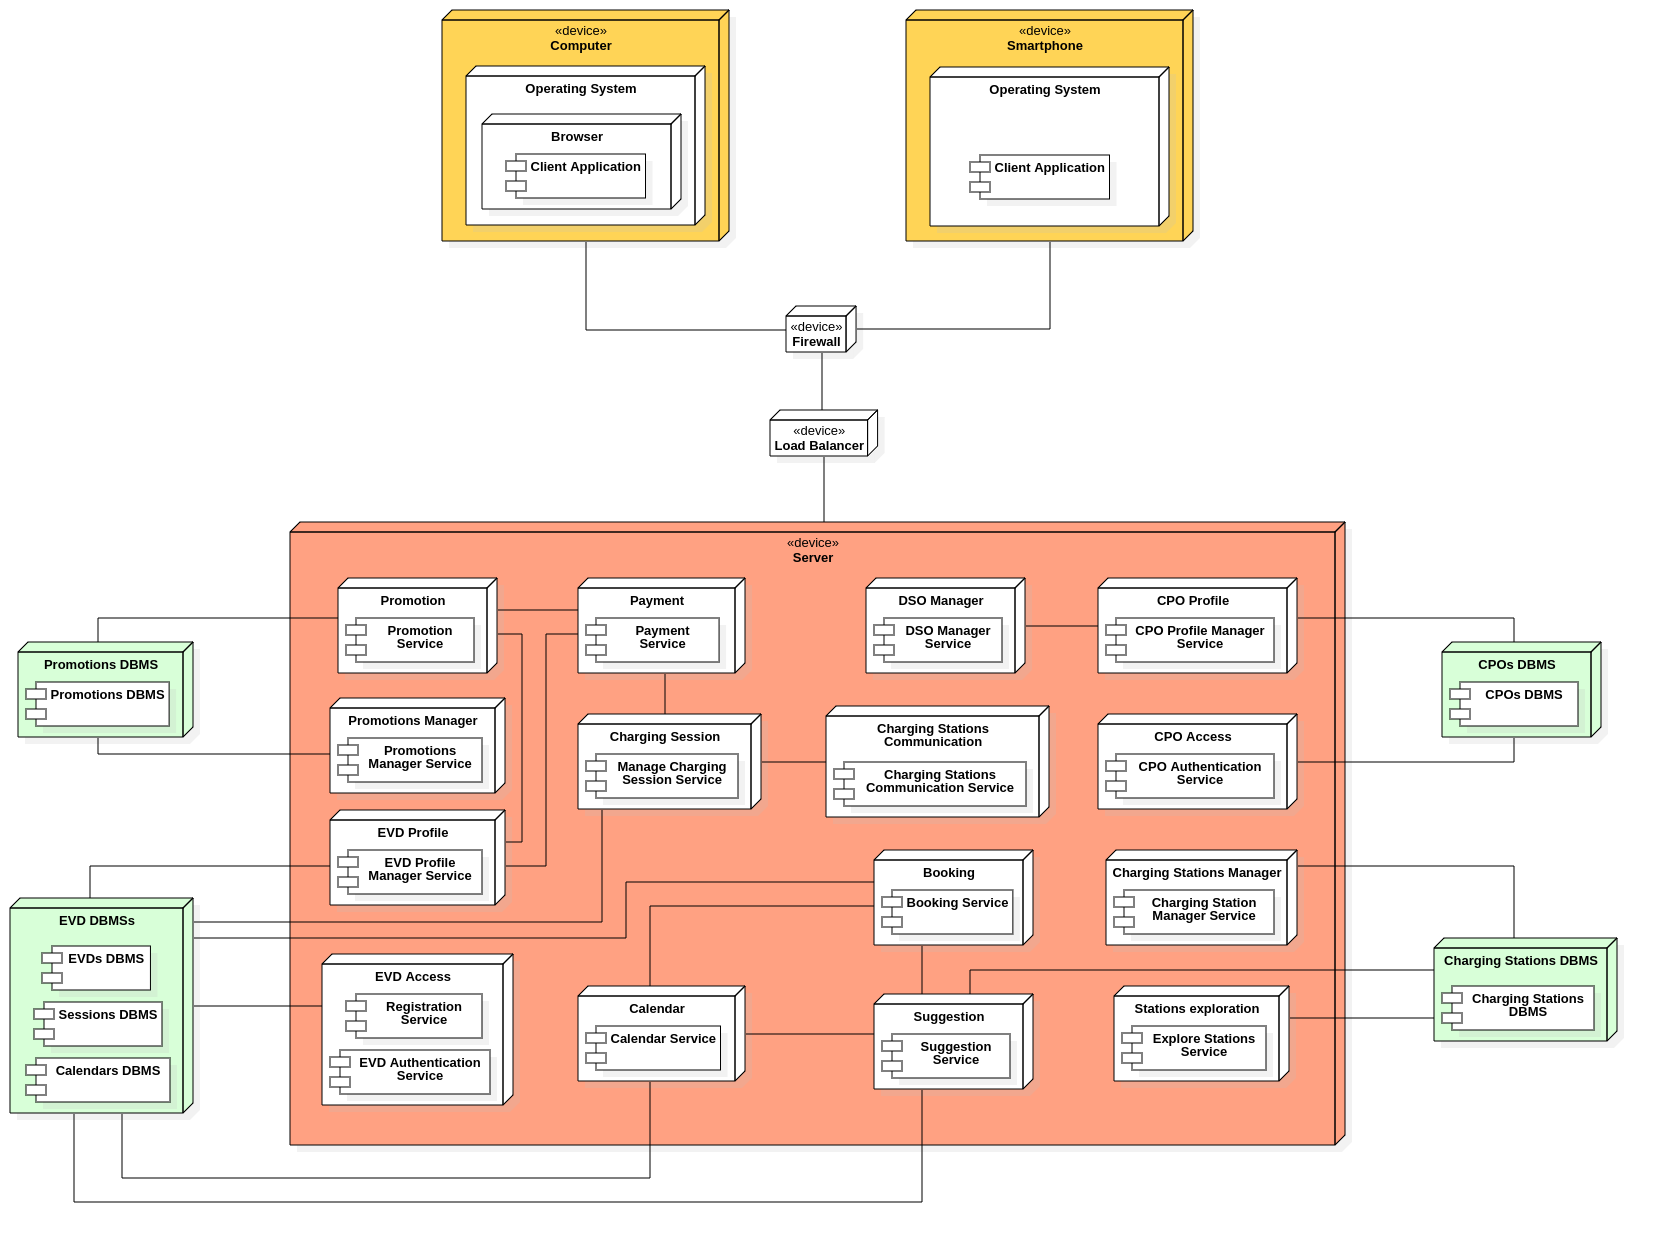
\includegraphics[width=1\linewidth]{DeploymentDiagram/deployment_diagram}
        \caption{Deployment diagram of the eMALL system.}
        \label{fig: depl_diagram}
    \end{center}
\end{figure}

\subsection{Connection to the server}
\label{subsec:connection_to_the_server}%
EVDs and CPOs can access to the \verb|eMALL| system from both PC and smartphone.
In the first case, it is necessary to use a browser in order to get the web page of the system.
In the second case, the client will use the application after having downloaded it from the smartphone's store (Android or iOS).
When requests are sent to the server, first they pass into the firewall, so to avoid eventual cyberattacks to the system,
and then they pass into the load balancer, so to optimize resource usage, improve performance, and increase availability of the several services.
Load balancer will distribute the requests, that are now ready to be handled by the \verb|eMALL| services.
It follows the corresponding part from the deployment diagram:
\begin{figure} [H]
    \begin{center}
        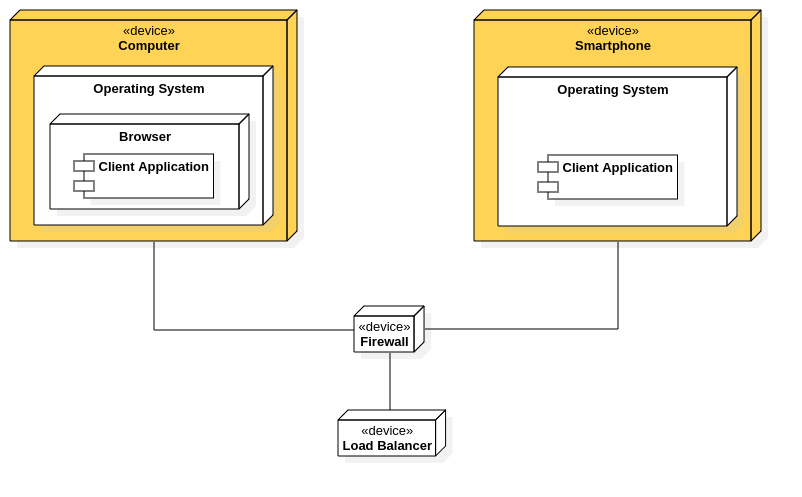
\includegraphics[width=0.7\linewidth]{DeploymentDiagram/connection}
        \caption{Connection to the server diagram.}
        \label{fig: connection}
    \end{center}
\end{figure}

\subsection{Promotions}
\label{subsec:promotions}%
Promotion DBMS is one of the four DBMS nodes that have been identified.
The choice of having divided it from other DBMS relies on the will to better scale the system:
in this way, in fact, it is easier to guarantee the availability
of other services that don't work with promotions, and maintenance sessions are facilitated too.
It has not been grouped with other DBMSs into the same node because \verb|Promotions DBMS| is used also by CPOs,
so the system needs to guarantee a high level of scalability in order to assure business functionalities to the companies.
\begin{figure} [H]
    \begin{center}
        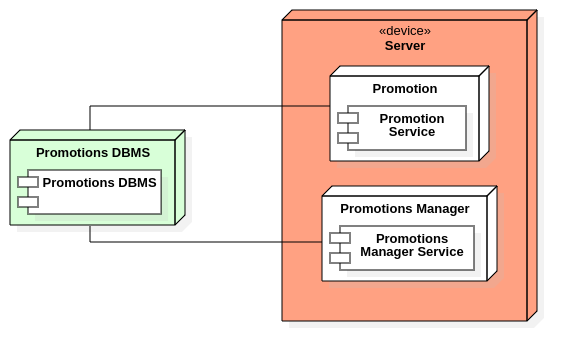
\includegraphics[width=0.6\linewidth]{DeploymentDiagram/promotion}
        \caption{Promotions managing diagram.}
        \label{fig: promotion}
    \end{center}
\end{figure}

\subsection{EVD interactions}
\label{subsec:evd_interactions}%
\begin{figure} [H]
    \begin{center}
        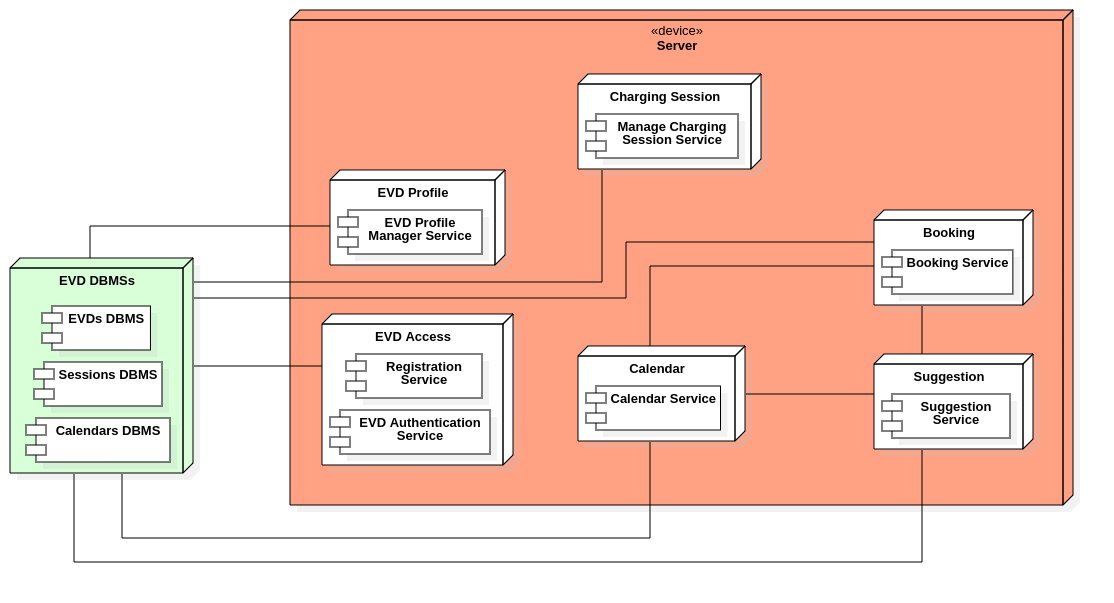
\includegraphics[width=\linewidth]{DeploymentDiagram/EVD_interactions}
        \caption{EVD interactions diagram.}
        \label{fig: evd_interactions}
    \end{center}
\end{figure}

\subsection{CPO DBMS}
\label{subsec:cpo_dbms}%
\begin{figure} [H]
    \begin{center}
        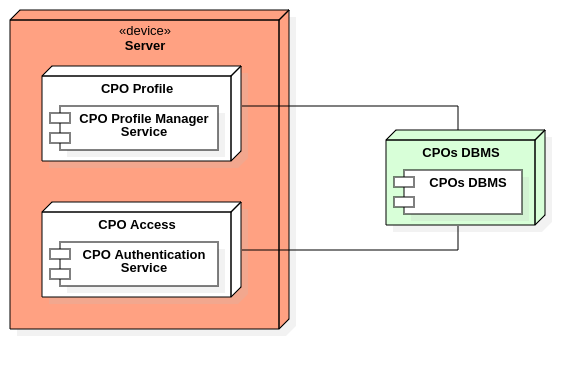
\includegraphics[width=0.6\linewidth]{DeploymentDiagram/CPO_DBMS}
        \caption{CPOs DBMS managing diagram.}
        \label{fig: cpo_dbms}
    \end{center}
\end{figure}

\subsection{Charging stations communication}
\label{subsec:charging_stations_communication}%
\begin{figure} [H]
    \begin{center}
        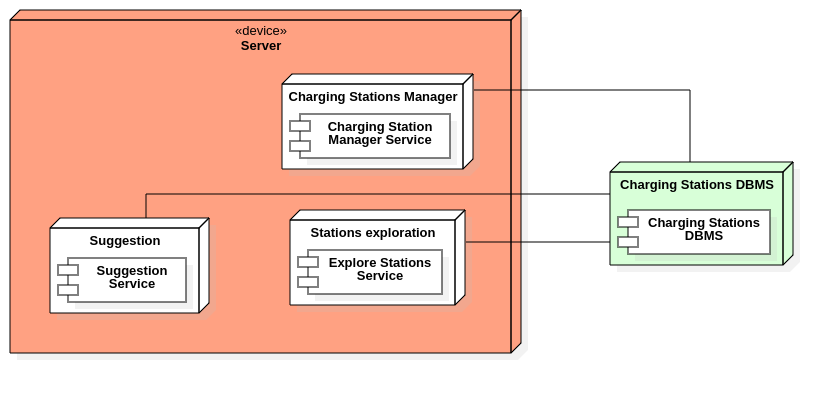
\includegraphics[width=0.85\linewidth]{DeploymentDiagram/charging_stations_communication}
        \caption{Charging stations communication diagram.}
        \label{fig: charing_stations_dbms}
    \end{center}
\end{figure}

\subsection{Services}
\label{subsec:services}%
\begin{figure} [H]
    \begin{center}
        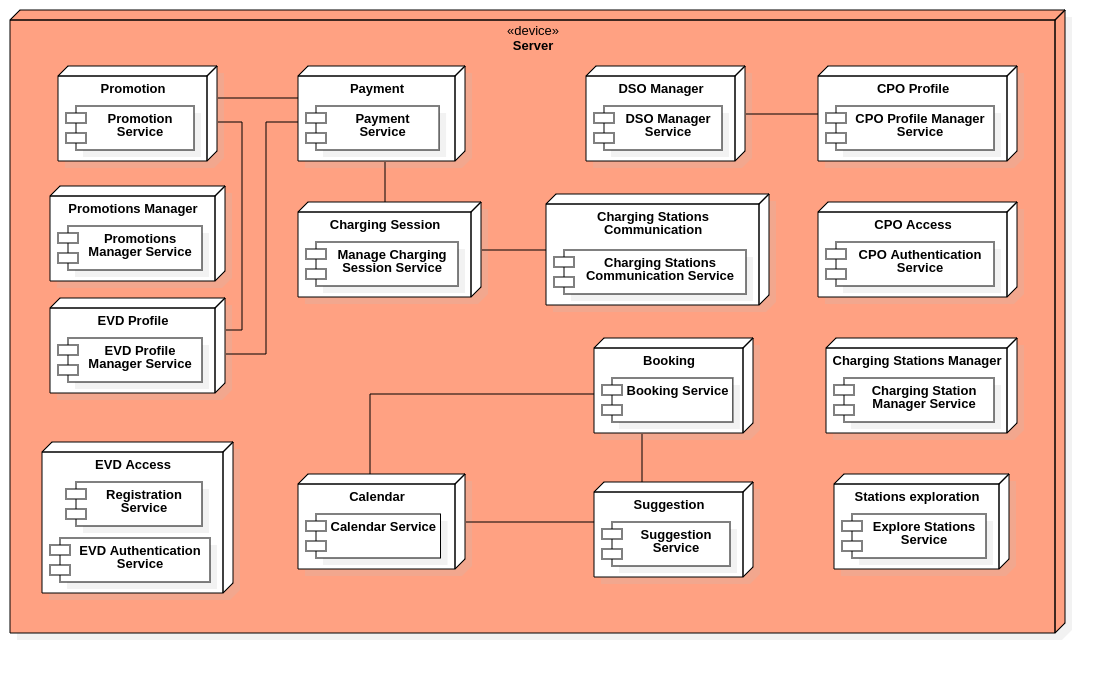
\includegraphics[width=\linewidth]{DeploymentDiagram/server}
        \caption{Server services diagram.}
        \label{fig: services}
    \end{center}
\end{figure}



\section{Runtime View}
\label{sec: runtime_view}%


\section{Component Interfaces}
\label{sec: component_interfaces}%


\section{Selected Architectural Styles and Patterns}
\label{sec: patterns}%


\section{Other Design Decisions}
\label{sec: other_design_decisions}%
